\textbf{aperiodischer Grenzfall:} $\omega'=0$\qquad keine Schwingung mehr

\subsection{harmonischer Oszillator}
\begin{wrapfigure}{r}{5cm}
    \captionsetup{type=figure}
    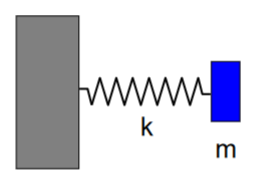
\includegraphics[width=4.5cm]{pictures/Oszillator.png}
    \caption{Oszillator}\label{fig:Oszillator}
\end{wrapfigure}

\[ F = -k\cd x = m\cdot a = m\cdot \ddot{x}\]
DGL lösen dann ist:
\begin{align*}
    x(t) &= x_0 \cdot \cos (w_o\cdot t + \alpha)\\
    v(t) &= -\omega_0 x_0 \sin(\omega_0t+\alpha)\\
    a(t) &= -\omega_0^2 \cos (\omega_0 t + \alpha) = -\omega_0^2 x(t)\\
    & \text{mit: } \omega^2 = \frac{k}{m} \quad \omega = \frac{2\pi}{T} \quad T=2\pi   \cdot \sqrt{\frac{m}{k}}\\
    & \text{komplex:}\\
    x(t)&= A\cdot e^{i(\omega t + \alpha)}\\
    v(t)&= i \cdot \omega \cdot A\cdot e^{i(\omega t + \alpha)} = \omega \cdot A\cdot e^{i(\omega t + \alpha + \frac{\pi}{2})}\qquad (i=e^{i \pi/2}) \\
    a(t)&= -\omega ^2 \cdot A\cdot e^{i(\omega t + \alpha)} = \omega ^2 \cdot A\cdot e^{i(\omega t + \alpha + \pi)}\\
\end{align*}

Die Realteile der komplexen Funktionen liefern die physikalischen Größen zum Zeitpunkt $t$.\\

\subsection{Erzwungene Schwingungen}
$F(t)=F_0\cos (\omega t)$... periodische äußere Kraft, $\omega_0^2=\frac{k}{m}$... Eigenfrequenz des Systems
\begin{align*}
    m\cdot a &= F(t) + F_F = F(t) -k\cdot x\\
    m\cdot \ddot{x} &= F(t) - k\cdot x\\
    \ddot{x}(t)&=\frac{F_0}{m}\cos(\omega t)-\omega_0^2 \cdot x
\end{align*}

\begin{samepage}
    \begin{wrapfigure}{r}{.4\textwidth}
        einsetzen in DGL\\
        $-\omega^2\cdot x_0\cdot e^{i\omega t} = \frac{F_0}{m}\cdot e^{i\omega t} - \omega_0^2 \cdot x_0 \cdot e^{i\omega t}$\\

        $\bm{\Rightarrow x_0=\frac{F_0}{m(\omega_0^2-\omega^2)}}$\\

        \textbf{Resonantzkatastrophe} bei $\omega_0$ da $x_0$ divergiert.
    \end{wrapfigure}
    \textbf{DGL mit komplexen Ansatz lösen:}\\
    \begin{align*}
        F(t) &= F_0\cdot e^{i\omega t}\\
        x(t) &=x_0 \cdot e^{i\omega t}\\
        \dot{x}(t) &= i\cdot \omega \cdot x_0 \cdot e^{i\omega t}\\
        \ddot{x}(t) &= - \omega^2 \cdot x_0 \cdot e^{i\omega t}
    \end{align*}
\end{samepage}



\subsection{Erzwungene, gedämpfte Schwingungen}
\begin{align*}
    m\cdot a &= F(t) + F_F + F_D = F(t) -k\cdot x - d\cdot v\\
    m\cdot \ddot{x} &= F(t) - k\cdot x -d \cdot \dot{x}
\end{align*}


